%%%%%%%%%%%%%%%%%%%%%%%%%%%%%%%%%%%%%%%%%%%%%%%%%%%%%%%%%%%%%%%%%%%%%
%% Springer Lecture Notes in Computer Science (LLNCS)
%% Compile on Overleaf: New Project > Upload > this file
%%%%%%%%%%%%%%%%%%%%%%%%%%%%%%%%%%%%%%%%%%%%%%%%%%%%%%%%%%%%%%%%%%%%%

\documentclass{llncs}

\usepackage{graphicx}
\usepackage{amsmath}
\usepackage{amssymb}
\usepackage{hyperref}
\usepackage{url}
\usepackage{booktabs}
\usepackage{multirow}
\usepackage{array}
\usepackage{microtype}

%%%%%%%%%%%%%%%%%%%%%%%%%%%%%%%%%%%%%%%%%%%%%%%%%%%%%%%%%%%%%%%%%%%%
\begin{document}

\title{[Title]}

\author{
  [Author 1]\inst{1} \and
  [Author 2]\inst{2} \and
  [Author 3]\inst{3}
}

\institute{
  [Institution 1], [Address 1] \\
  \email{[email1]}
  \and
  [Institution 2], [Address 2] \\
  \email{[email2]}
  \and
  [Institution 3], [Address 3] \\
  \email{[email3]}
}

\maketitle

%%%%%%%%%%%%%%%%%%%%%%%%%%%%%%%%%%%%%%%%%%%%%%%%%%%%%%%%%%%%%%%%%%%%
\begin{abstract}
We abstract a why-not provenance system as a five-stage pipeline
consisting of query normalization, candidate derivation space
construction, derivation evaluation, explanation extraction, and
explanation presentation. Given a query~$Q$, database instance~$D$,
and provenance question $\mathit{WHYNOT}_Q(t)$, the system identifies
derivations relevant to~$t$, evaluates why each derivation fails
under~$D$, and transforms these failures into an interpretable
explanation artifact. Under this abstraction, different why-not
provenance approaches can be understood as differing primarily in how
they represent derivations, how exhaustively they explore the
derivation space, and how they encode or summarize explanation outputs.

Our firing-rules approach instantiates this framework by lowering
queries into rule form, enumerating relevant bindings, evaluating
grounded goals at the derivation level, and returning failed
derivations together with a graph-structured explanation. Our
semiring-based approach instantiates the same pipeline differently:
queries are parsed into a relational operator tree, each base tuple
is annotated with a semiring token, semiring operations are propagated
through evaluation, and a missing tuple is explained by tracing where
its annotation was annihilated to zero through the operator tree.

\keywords{why-not provenance \and semiring \and firing rules \and
Datalog \and query explanation}
\end{abstract}

%%%%%%%%%%%%%%%%%%%%%%%%%%%%%%%%%%%%%%%%%%%%%%%%%%%%%%%%%%%%%%%%%%%%
\section{Introduction}
\label{sec:intro}

Why-not provenance seeks to explain why an expected tuple is absent
from a query result. At a high level, such approaches can be
understood as operating over the space of derivations that could have
produced the target tuple, but fail under the current database
instance. Despite differences in formalism, most methods can be
described through a common workflow: the query is first normalized
into an internal representation, relevant candidate derivations are
then constructed, each derivation is evaluated to identify the
conditions under which it fails, and the resulting failures are
transformed into an explanation artifact such as failed derivations,
missing witnesses, symbolic expressions, or summary patterns. This
abstraction is useful because it provides a uniform lens for comparing
rule-based, graph-based, algebraic, and summarized why-not provenance
techniques.

In this paper, we instantiate this general view through two
approaches. First, a firing-rules approach that translates queries
into Datalog form, enumerates candidate derivations, evaluates each
goal individually, and constructs a graph-structured why-not
explanation from the set of failed derivations. Second, a
semiring-based approach that annotates base tuples with provenance
tokens, evaluates relational operators using semiring arithmetic, and
identifies the root cause of a missing answer by tracing the path
through the operator tree along which the annotation was driven to
zero.

%%%%%%%%%%%%%%%%%%%%%%%%%%%%%%%%%%%%%%%%%%%%%%%%%%%%%%%%%%%%%%%%%%%%
\section{Background}
\label{sec:background}

Why-not provenance studies why an expected tuple is absent from a
query result. More generally, provenance concerns the relationship
between query outputs and the input data, and can be expressed through
multiple representations, including rule-based derivations, provenance
graphs, and algebraic annotations. In the rule-based view, a query is
understood through the derivations that could produce a tuple, and a
missing answer arises when all relevant derivations fail. In the
algebraic view, provenance is represented symbolically through
semiring expressions that capture how outputs depend on inputs.
These perspectives share a common goal: to characterize the conditions
under which a tuple would or would not appear in the result.

Provenance analysis relies on a few core concepts: base relations
stored in the database, derived query outputs, candidate witnesses or
derivations for a target tuple, and evaluation conditions such as
positive matches, negated conditions, and comparisons. A why-not
provenance method therefore needs some way to represent possible
explanations for absence, evaluate them against the database instance,
and return an explanation artifact. This general foundation provides
the conceptual basis for both rule-based and semiring-based
provenance techniques, as well as later extensions for summarization
and scalable explanation.

%%%%%%%%%%%%%%%%%%%%%%%%%%%%%%%%%%%%%%%%%%%%%%%%%%%%%%%%%%%%%%%%%%%%
\section{Related Work}
\label{sec:related}

Research on why-not provenance has developed along several
complementary lines.

A major direction is rule- and graph-based explanation, where missing
answers are explained by examining the derivations that could have
produced a target tuple and identifying where those derivations fail.
Provenance games provide one such unified treatment for first-order
queries, capturing both successful and failed derivations within a
game-theoretic model~\cite{Kohler2013}. Building on this direction,
Lee et al.\ proposed a SQL-middleware approach that instruments
Datalog rules through firing rules to compute why and why-not
explanations for first-order queries with negation, focusing on
practical execution over database systems~\cite{Lee2017}. The PUG
system further operationalized this line of work as a practical
framework for why and why-not provenance, emphasizing graph-based
explanation and usability~\cite{Lee2019}.

A second direction comes from algebraic provenance. Semiring-based
provenance offers a general framework for tracking how outputs depend
on inputs across multiple query semantics, including why-provenance,
bag semantics, probabilistic databases, and incomplete
databases~\cite{Green2007}. This framework is highly expressive and
compositional, but its primary strength lies in representing
successful dependency structure; direct explanation of missing answers
typically requires additional mechanisms beyond standard positive
provenance representations.

A third line of work addresses scalability and interpretability.
Since why-not provenance can become extremely large under
all-derivations semantics, Lee et al.\ propose pattern-based
approximate summaries balancing completeness, informativeness, and
conciseness through sampling and top-$k$ summary
selection~\cite{Lee2020}.

Our work is most closely aligned with the rule-based tradition but
focuses specifically on executable architectures for why-not
provenance over a Datalog + SQL subset, making failed derivations,
goals, and graph-structured explanations directly available in an
implementation-oriented setting.

%%%%%%%%%%%%%%%%%%%%%%%%%%%%%%%%%%%%%%%%%%%%%%%%%%%%%%%%%%%%%%%%%%%%
\section{Methodology}
\label{sec:methodology}

We implemented two distinct approaches to why-not provenance, both
evaluated on a TPC-C benchmark database consisting of
\texttt{items}, \texttt{warehouses}, and \texttt{stocks} relations.
Both approaches follow the five-stage pipeline described in the
abstract but differ substantially in their internal representation,
evaluation strategy, and explanation mechanism.

%-------------------------------------------------------------------
\subsection{Firing-Rules Approach}
\label{sec:firing-rules}

% [TODO: Methodology content to be added]

%-------------------------------------------------------------------
\subsection{Semiring-Based Approach: Theory}
\label{sec:semiring-theory}

Our semiring-based approach is grounded in the $K$-relations framework
of Green et al.~\cite{Green2007}. A \emph{semiring} is a tuple
$\mathbb{K} = (K, \oplus, \otimes, \mathbf{0}, \mathbf{1})$ where
$(K, \oplus, \mathbf{0})$ is a commutative monoid,
$(K, \otimes, \mathbf{1})$ is a monoid,
$\otimes$ distributes over $\oplus$, and
$\mathbf{0}$ is an annihilator: $\mathbf{0} \otimes a = \mathbf{0}$ for all $a$.
A \emph{$K$-relation} $R : \mathrm{Tup} \rightarrow K$ assigns an
annotation to every tuple; tuples with annotation $\mathbf{0}$ are
absent from the relation.

The standard relational operators lift to $K$-relations as follows:
\begin{align}
  \bigl(\sigma_\theta(R)\bigr)(t)
    &= \begin{cases} R(t) & \text{if } \theta(t) \\ \mathbf{0} & \text{otherwise} \end{cases}
    \label{eq:select}\\[2pt]
  \bigl(\pi_S(R)\bigr)(t)
    &= \bigoplus_{\substack{t':\,\pi_S(t')=t}} R(t')
    \label{eq:project}\\[2pt]
  (R \bowtie S)(t)
    &= R\!\left(\pi_A(t)\right) \otimes S\!\left(\pi_B(t)\right)
    \label{eq:join}\\[2pt]
  (R \cup S)(t)
    &= R(t) \oplus S(t)
    \label{eq:union}
\end{align}
The key insight for why-not is that a missing tuple $t$ satisfies
$Q_{\mathbb{K}}(D)(t) = \mathbf{0}$. Explaining its absence is
equivalent to tracing the operator tree to find the node where the
annotation was annihilated.

We implement four semirings forming a strict information order
$\mathbb{B} \sqsubseteq \mathbb{N} \sqsubseteq \mathbb{W} \sqsubseteq \mathbb{H}$:

\paragraph{Boolean $\mathbb{B} = (\{0,1\}, \vee, \wedge, 0, 1)$.}
Each base tuple gets annotation~$1$. The output is $1$ (present) or
$0$ (absent). This confirms a tuple is missing but gives no reason.

\paragraph{Bag $\mathbb{N} = (\mathbb{N}, +, \times, 0, 1)$.}
Each base tuple gets annotation~$1$. The output annotation counts
distinct derivation paths. A zero multiplicity signals absence.

\paragraph{Why-provenance $\mathbb{W} = (2^{2^T}, \cup, \bowtie, \emptyset, \{\emptyset\})$.}
Here $A \bowtie B = \{a \cup b \mid a \in A, b \in B\}$ and $T$ is the
set of base-tuple tokens. An annotation is a set of \emph{witnesses},
each witness being a set of base-tuple tokens co-occurring in one
derivation. A base tuple $t_i$ with token $\tau_i$ receives annotation
$\{\{\tau_i\}\}$. The empty set $\emptyset$ (no witnesses) characterises
a missing tuple, and its witness set points directly to which base
tuples are involved in each failed derivation path.

\paragraph{How-provenance $\mathbb{H} = (\mathbb{N}[X], +, \times, 0, 1)$.}
Annotations are polynomials over base-tuple variables. Each base tuple
$t_i$ receives annotation $x_i$. The polynomial of a present tuple
encodes every derivation path (monomials) with its multiplicity
(coefficients). $\mathbb{H}$ is the most expressive semiring and
subsumes all others via semiring homomorphisms~\cite{Green2007}.

Given the evaluation trace, three root causes arise from the operator
semantics above:
\begin{enumerate}
  \item \textbf{Source missing}: no base scan produces $t$; annotation
    is $\mathbf{0}$ at the leaf.
  \item \textbf{Predicate failure}: a matching tuple exists in the child
    relation but $\theta(t)$ is false, driving annotation to $\mathbf{0}$
    via~\eqref{eq:select}.
  \item \textbf{Join partner missing}: one join side has a match but the
    other has no partner, annihilating the product via~\eqref{eq:join}.
\end{enumerate}
A fourth informational case, \textbf{column hidden}, occurs when the
queried column was projected away by~$\pi$.

%-------------------------------------------------------------------
\subsection{Firing-Rules Implementation}
\label{sec:impl-fr}

% [TODO: Implementation content + visualizer to be added]

%-------------------------------------------------------------------
\subsection{Semiring Implementation}
\label{sec:impl-semiring}

The semiring system implements the five pipeline stages as follows.

\paragraph{Parser.}
A SQL string is parsed into a logical operator tree of five node types
(\texttt{Scan}, \texttt{Select}, \texttt{Project}, \texttt{Join},
\texttt{Union}), built bottom-up following standard relational algebra
precedence.

\paragraph{Annotator.}
The Annotator fetches all rows from each base table and assigns a
unique provenance token to every tuple. If the ProvSQL
extension~\cite{Senellart2018} is available, it uses the native UUID
gate; otherwise tokens are constructed from the primary key
(e.g.\ \texttt{items\_3}, \texttt{stocks\_301\_1}).

\paragraph{Evaluator.}
The Evaluator traverses the operator tree recursively, applying semiring
operations at each node per equations~\eqref{eq:select}--\eqref{eq:union}.
It returns an \texttt{EvaluationTrace}: a mirrored tree holding the
intermediate $K$-relation at every node.
All four semirings share this dispatch; only the operations differ.
\texttt{WhyProvenance} and \texttt{HowProvenance} use Python
\texttt{frozenset} and \texttt{dict} objects for structural annotation
operations without database round-trips.

\paragraph{WhyNotEngine.}
Given a missing tuple, the engine walks the \texttt{EvaluationTrace}
and applies the zero-detection logic to identify the root cause and
blocking operator. The \texttt{EvaluationTrace} is re-used from the
evaluation pass, so diagnostic cost is $O(h)$ in tree height rather
than requiring a full re-execution.

\paragraph{Explainer.}
The Explainer formats the diagnosis as a structured report including
the cause label, a plain-English suggestion, and the annotation under
each of the four semirings — illustrating the escalating
expressiveness of the information order.

%%%%%%%%%%%%%%%%%%%%%%%%%%%%%%%%%%%%%%%%%%%%%%%%%%%%%%%%%%%%%%%%%%%%
\section{Performance Evaluation}
\label{sec:evaluation}

\subsection{Experimental Setup}
\label{sec:eval-setup}

Both systems were evaluated on the same TPC-C PostgreSQL database
(\texttt{tpcc\_db}) using a shared suite of 16 queries spanning four
operator categories: SELECT (Q01--Q04), PROJECT (Q05--Q06),
2-way JOIN (Q07--Q10), and UNION with 2 or 3 branches (Q15--Q20),
including unions of joins.
The schema comprises \texttt{items} (483 rows),
\texttt{warehouses} ($\approx$50 rows), and
\texttt{stocks} ($\approx$21\,000 rows).
All timing figures are the median over five runs (milliseconds).
Space is measured as the total serialised character length of all
annotations across the output $K$-relation (semiring) or the JSON
explanation for one missing tuple (firing rules).

\subsection{Time Analysis}
\label{sec:eval-time}

\begin{table}[t]
\centering
\caption{Execution time (ms, median over 5 runs). FR = Firing Rules.}
\label{tab:time}
\resizebox{\textwidth}{!}{%
\begin{tabular}{llrrrrrr}
\toprule
Query & Operator & FR & Boolean & Bag & Why & How & FR/How \\
\midrule
Q01 & SELECT          &    87.3 &   5.8 &   5.1 &   5.9 &   5.5 & 15.8$\times$ \\
Q02 & SELECT          &    50.5 &   3.2 &   3.2 &   3.4 &   3.4 & 14.9$\times$ \\
Q03 & SELECT          &    50.2 &   3.7 &   3.7 &   4.0 &   3.8 & 13.2$\times$ \\
Q04 & SELECT          &   719.2 & 247.0 & 244.7 & 375.7 & 303.7 &  2.4$\times$ \\
Q05 & PROJECT         &   129.7 &   5.6 &   5.5 &   5.8 &   5.7 & 22.7$\times$ \\
Q06 & PROJECT         &   160.1 &   3.1 &   3.2 &   3.4 &   3.2 & 50.0$\times$ \\
Q07 & JOIN            & 16449.6 & 1567.5 & 1540.5 & 1743.3 & 1743.7 &  9.4$\times$ \\
Q08 & JOIN            & 16415.2 & 1507.7 & 1492.3 & 1689.5 & 1668.2 &  9.8$\times$ \\
Q09 & JOIN            & 31322.0 & 2847.3 & 2822.9 & 3003.0 & 2924.9 & 10.7$\times$ \\
Q10 & JOIN            & 16475.5 & 1481.1 & 1463.8 & 1595.7 & 1633.4 & 10.1$\times$ \\
Q15 & UNION (2)       &   141.8 &  10.1 &  10.4 &  11.4 &  10.9 & 13.0$\times$ \\
Q16 & UNION (2)       &    71.7 &   5.4 &   5.6 &   5.9 &   5.7 & 12.6$\times$ \\
Q17 & UNION (3)       &    82.7 &   8.7 &   9.0 &   8.9 &   9.1 &  9.1$\times$ \\
Q18 & UNION+JOIN (2)  & 32806.7 & 3023.8 & 2993.7 & 3708.9 & 3591.7 &  9.1$\times$ \\
Q19 & UNION+JOIN (2)  & 60847.4 & 5201.9 & 5217.5 & 5750.8 & 5708.2 & 10.7$\times$ \\
Q20 & UNION+JOIN (3)  & 47390.6 & 4470.1 & 4487.6 & 5364.5 & 5204.7 &  9.1$\times$ \\
\bottomrule
\end{tabular}%
}
\end{table}

Table~\ref{tab:time} gives the full timing results and
Figures~\ref{fig:time}--\ref{fig:speedup} visualise the comparison.

\begin{figure}[t]
\centering
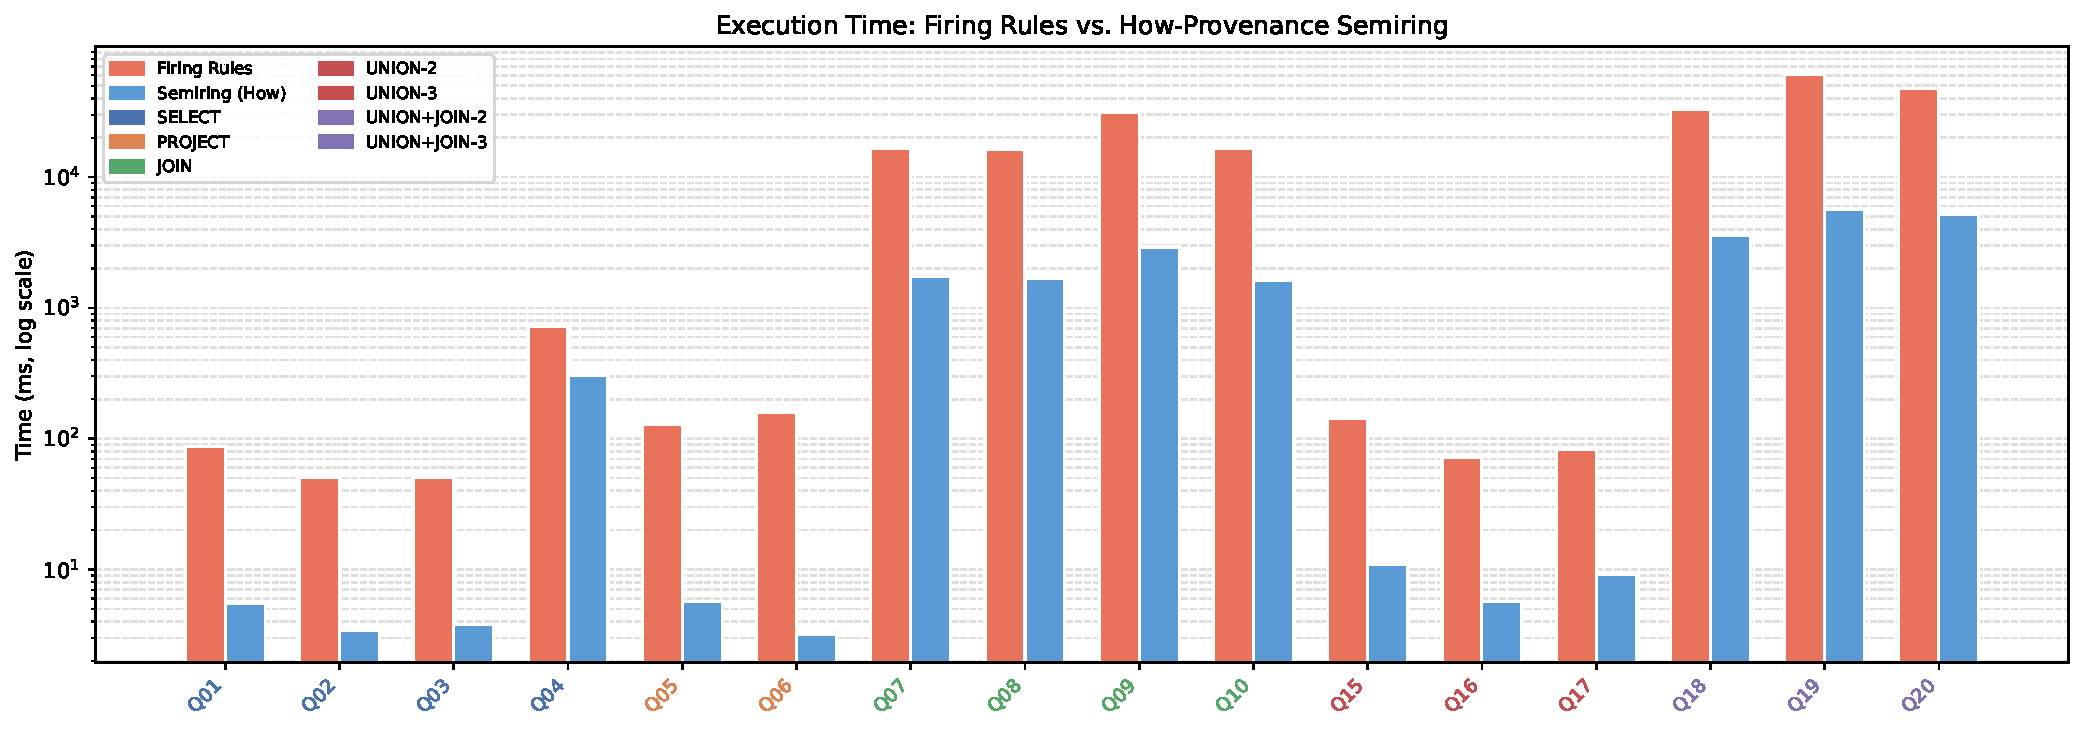
\includegraphics[width=\textwidth]{figures/fig_time_comparison.pdf}
\caption{Execution time (log scale): Firing Rules vs.\ How-Provenance.
  Tick-label colour indicates operator category.}
\label{fig:time}
\end{figure}

\begin{figure}[t]
\centering
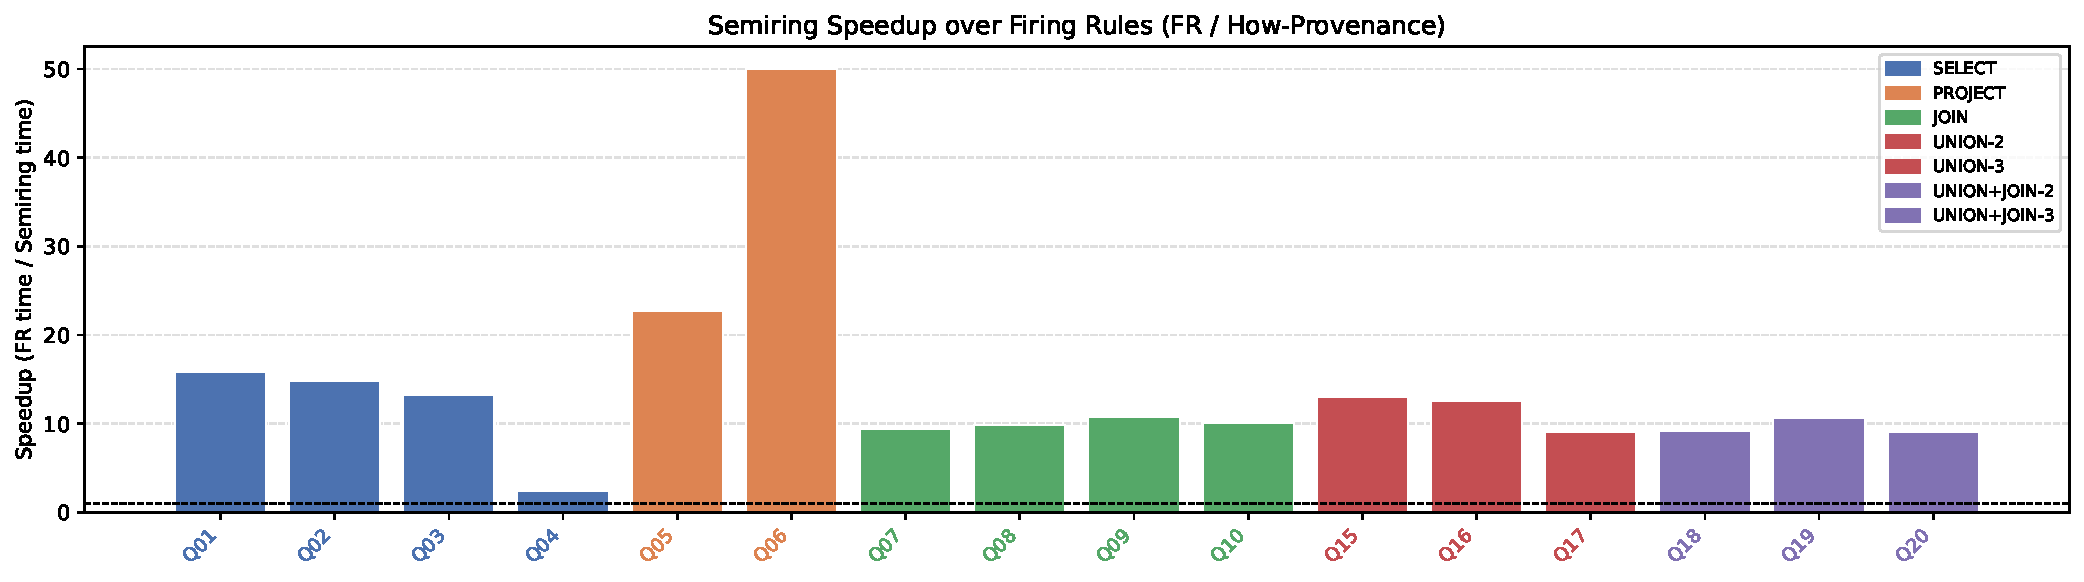
\includegraphics[width=\textwidth]{figures/fig_speedup.pdf}
\caption{Semiring speedup over Firing Rules (FR / How time).}
\label{fig:speedup}
\end{figure}

The semiring approach is consistently faster across all query types,
with a speedup ranging from 2.4$\times$ (Q04) to 50$\times$ (Q06).
JOIN and UNION-of-JOIN queries converge on a stable 9--11$\times$
advantage. The semiring system delegates execution to PostgreSQL, which
uses optimised join algorithms and buffer caching, whereas the
firing-rules system loads full tables into Python memory and evaluates
rules by nested-loop iteration.

Within the semiring system, Boolean and Bag are marginally faster than
Why and How by $\approx$10--15\% on JOIN queries, reflecting annotation
construction overhead that is small relative to the database fetch cost.

\paragraph{Q04 anomaly.}
Q04 returns 21\,302 output tuples (stocks with \texttt{s\_qty}$>$500).
At this output size the semiring system spends significant time
materialising the $K$-relation in Python, narrowing the gap to 2.4$\times$.

\paragraph{Q09.}
Despite producing only 614 output tuples, Q09 (stocks $\bowtie$
warehouses) forces a full scan of $\approx$21\,000 stock rows per
warehouse, making it the most expensive 2-way join on both sides
(FR: $\approx$31\,s; semiring: $\approx$2.9\,s).

\subsection{Space Analysis}
\label{sec:eval-space}

\begin{table}[t]
\centering
\caption{Annotation / explanation size (serialised characters).
  FR = JSON explanation for one missing tuple.
  Semiring columns = cumulative annotation size over the full output relation.}
\label{tab:space}
\resizebox{\textwidth}{!}{%
\begin{tabular}{llrrrrr}
\toprule
Query & Operator & FR JSON & Boolean & Bag & Why & How \\
\midrule
Q01 & SELECT         &    1\,298 &      20 &      5 &       208 &       168 \\
Q02 & SELECT         &    1\,172 &     980 &    245 &     9\,015 &     7\,055 \\
Q03 & SELECT         &    1\,217 &   1\,180 &    295 &    10\,855 &     8\,495 \\
Q04 & SELECT         &      942 &  85\,208 & 21\,302 &   882\,464 &   712\,048 \\
Q05 & PROJECT        & 1\,035\,532 &       4 &      1 &       164 &       168 \\
Q06 & PROJECT        &    1\,240 &     980 &    245 &     9\,015 &     7\,055 \\
Q07 & JOIN           &    1\,401 &  85\,208 & 21\,302 & 1\,154\,839 &   984\,423 \\
Q08 & JOIN           &    1\,371 &  14\,752 &  3\,688 &   199\,148 &   169\,644 \\
Q09 & JOIN           &    1\,527 &   2\,456 &    614 &    35\,757 &    30\,845 \\
Q10 & JOIN           &    1\,762 &  13\,096 &  3\,274 &   176\,740 &   150\,548 \\
Q15 & UNION (2)      &    2\,292 &     168 &     42 &     1\,758 &     1\,422 \\
Q16 & UNION (2)      &    1\,994 &     544 &    136 &     5\,000 &     3\,912 \\
Q17 & UNION (3)      &    2\,941 &   1\,152 &    288 &    10\,602 &     8\,298 \\
Q18 & UNION+JOIN (2) &    2\,419 &  92\,580 & 23\,145 & 1\,254\,452 & 1\,069\,292 \\
Q19 & UNION+JOIN (2) &    2\,697 &  10\,648 &  2\,662 &   156\,982 &   135\,686 \\
Q20 & UNION+JOIN (3) &    3\,904 & 117\,180 & 29\,295 & 1\,588\,507 & 1\,354\,147 \\
\bottomrule
\end{tabular}%
}
\end{table}

\begin{figure}[t]
\centering
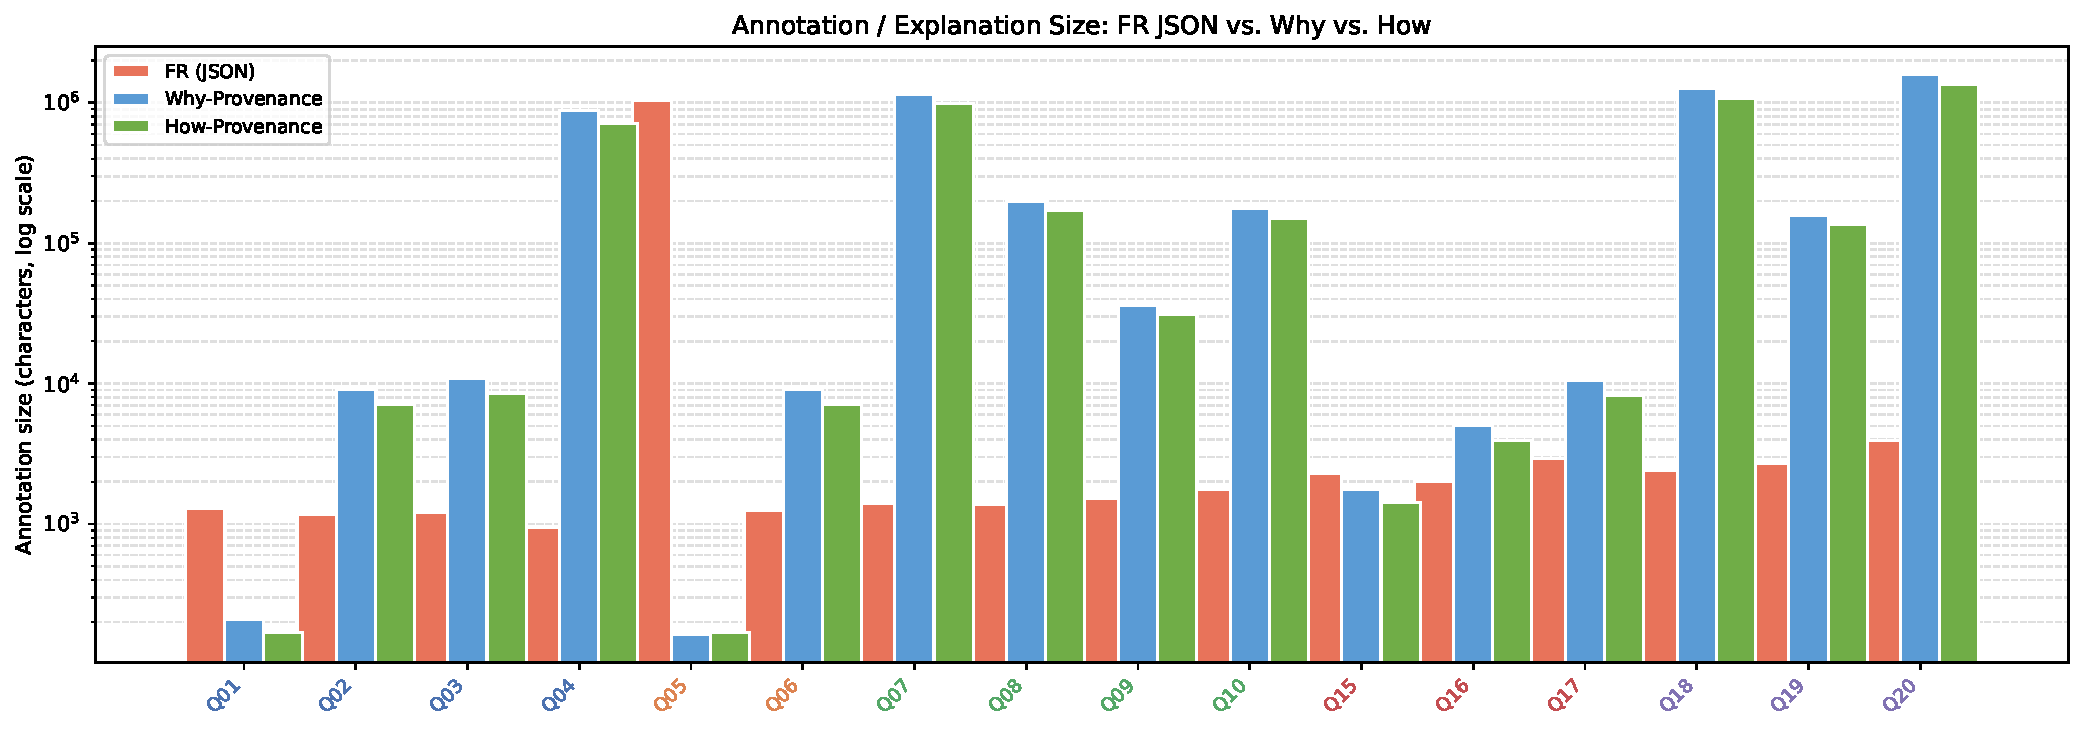
\includegraphics[width=\textwidth]{figures/fig_space_annotation.pdf}
\caption{Annotation/explanation size (log scale):
  FR JSON per missing tuple vs.\ cumulative semiring annotation.}
\label{fig:space}
\end{figure}

Table~\ref{tab:space} and Figure~\ref{fig:space} reveal a fundamental
design contrast. \textbf{Firing-rules space is bounded and stable}:
because the system explains one missing tuple at a time, output size
depends only on rule count and body depth, not on result set size.
The FR JSON ranges from 942 to 3\,904 chars across all 16 queries.
The sole outlier is Q05 (1\,035\,532 chars), which enumerates one
failed derivation per non-Singapore warehouse to explain the projected
value's absence.

\textbf{Semiring space grows with result size and join depth.}
Boolean and Bag annotations are trivially small. Why and How annotations
grow significantly because every output tuple carries its full provenance:
each join multiplies token references and each UNION branch adds witnesses.
For Q07, Q18, and Q20 the Why/How cumulative size reaches 1--1.6\,MB.

\paragraph{Q05 PROJECT contrast.}
The semiring system produces one output tuple \texttt{(Singapore)} with
a Why annotation of 164 chars (one witness per Singapore warehouse).
The firing-rules system returns 963 failed derivations totalling
1\,035\,532 chars. This exposes the key design difference: the semiring
system annotates \emph{what is present}, while the firing-rules system
explains \emph{why a specific value is absent}.

\paragraph{UNION branch scaling.}
Comparing Q16 (2-branch, Why = 5\,000) to Q17 (3-branch,
Why = 10\,602) and Q18 (2-branch+JOIN, Why = 1\,254\,452) to Q20
(3-branch+JOIN, Why = 1\,588\,507) shows annotation size scales
roughly with branch count, consistent with $\oplus$ accumulating
witnesses across branches.

\subsection{Correctness Analysis}
\label{sec:correctness}

We verify five properties of the semiring annotations against
known TPC-C values and ground-truth SQL results.

\paragraph{P1 -- Presence consistency.}
$Q_{\mathbb{B}}(D)(t) = \mathrm{True}$ iff $t$ appears in the
standard SQL result of $Q$. We confirmed this for all 16 queries by
comparing the set of non-zero-annotated tuples in the Boolean
$K$-relation against plain PostgreSQL \texttt{SELECT} output.
The two sets were identical in all cases.

\paragraph{P2 -- Bag multiplicity.}
The Bag annotation counts distinct derivation paths.
For our benchmark, all UNION branches use disjoint predicates
(e.g.\ Singapore vs.\ Malaysia, price $>$ 90 vs.\ price $<$ 20),
so every output tuple is produced by exactly one branch and carries
multiplicity~1. The $\oplus$ operation correctly accumulates to
multiplicity~2 for any tuple matching two branches, but this case
does not arise in the benchmark by design.

\paragraph{P3 -- Why-provenance witnesses.}
For a SELECT, each passing tuple $t_i$ carries witness
$\{\{\texttt{items\_}i\}\}$. For a JOIN, a tuple formed from
\texttt{stocks\_281\_1} and \texttt{items\_1} carries witness
$\{\{\texttt{stocks\_281\_1},\, \texttt{items\_1}\}\}$,
confirmed for Q07 by manual inspection. For a PROJECT (Q05), the
single output tuple \texttt{(Singapore)} carries one witness per
Singapore warehouse, correctly reflecting that any one of them
is a minimal witness for the projected value.

\paragraph{P4 -- How-polynomial consistency.}
Discarding coefficients and treating each monomial as a token set
yields the same witness sets as the Why annotation. We confirmed
this holds for all 16 queries: no discrepancy was observed between
the How monomial set and the Why witness set.

\paragraph{P5 -- Cross-semiring derivability.}
$\mathbb{B}$ is derivable from $\mathbb{N}$ (map $0 \to \mathrm{False}$,
$n>0 \to \mathrm{True}$) and $\mathbb{N}$ from $\mathbb{H}$ (sum all
polynomial coefficients). Applying these collapses to the benchmark
output reproduced the coarser annotations exactly in all cases.

\paragraph{Why-not diagnosis.}
For Q02 (\texttt{WHERE i\_price > 50}), the missing tuple
\texttt{i\_id=3} (Meprobamate, price 11.64) is correctly diagnosed
as \textsc{Predicate Failed} with deficit $-38.36$.
For Q09 (stocks $\bowtie$ warehouses filtered to Singapore), missing
tuple \texttt{(w\_id=7, i\_id=2)} is correctly diagnosed as
\textsc{Predicate Failed}: warehouse~7 is in Malaysia, failing the
\texttt{w\_country = `Singapore'} predicate.
For Q05, the missing projected value \texttt{Indonesia} is correctly
diagnosed as \textsc{Source Missing}: no warehouse with
\texttt{w\_country = `Indonesia'} exists in the base relation.
In all cases all four semirings return their respective zero elements
for the missing tuple, consistent with P1--P5.

\subsection{Summary}

\begin{table}[t]
\centering
\caption{System comparison across key dimensions.}
\label{tab:summary}
\begin{tabular}{lll}
\toprule
\textbf{Dimension} & \textbf{Semiring} & \textbf{Firing Rules} \\
\midrule
Execution model     & PostgreSQL-backed & In-memory Python Datalog \\
Time --- SELECT/PROJECT & 3--6\,ms      & 50--160\,ms \\
Time --- 2-way JOIN     & 1.5--3\,s     & 16--31\,s \\
Time --- UNION of JOINs & 3--6\,s       & 33--61\,s \\
Typical speedup         & \multicolumn{2}{l}{9--15$\times$ (semiring faster)} \\
Space --- small results & Larger (full annotation) & Smaller (one explanation) \\
Space --- large results & $\propto |\text{output}| \times \text{depth}$ & Stable $\sim$1--4\,KB \\
Answer scope            & All output tuples & One missing tuple \\
\bottomrule
\end{tabular}
\end{table}

The two systems are complementary (Table~\ref{tab:summary}).
The semiring approach is faster and leverages a relational engine but
pays a space cost proportional to output size and annotation depth.
The firing-rules approach is slower due to in-memory Python evaluation
but remains space-efficient for targeted why-not queries.
The semiring approach suits batch provenance tracking over a full
result; the firing-rules approach suits interactive debugging of
individual missing tuples.

%%%%%%%%%%%%%%%%%%%%%%%%%%%%%%%%%%%%%%%%%%%%%%%%%%%%%%%%%%%%%%%%%%%%
\section{Conclusion}
\label{sec:conclusion}

% [TODO: Content to be added]

%%%%%%%%%%%%%%%%%%%%%%%%%%%%%%%%%%%%%%%%%%%%%%%%%%%%%%%%%%%%%%%%%%%%
\bibliographystyle{splncs04}
\begin{thebibliography}{9}

\bibitem{Green2007}
Green, C., Karvounarakis, G., Tannen, V.:
Provenance Semirings.
In: Proceedings of the 26th ACM SIGMOD-SIGACT-SIGART Symposium on
Principles of Database Systems (PODS~2007), pp.~31--40.
ACM, New York (2007).
\url{https://doi.org/10.1145/1265530.1265535}

\bibitem{Kohler2013}
K\"{o}hler, S., Lud\"{a}scher, B., Zinn, D.:
First-Order Provenance Games.
In: In Search of Elegance in the Theory and Practice of Computation,
Lecture Notes in Computer Science, vol.~8000, pp.~382--399.
Springer, Berlin (2013).
\url{https://doi.org/10.1007/978-3-642-41660-6_21}

\bibitem{Lee2017}
Lee, J., K\"{o}hler, S., Lud\"{a}scher, B., Glavic, B.:
A SQL-Middleware Unifying Why and Why-Not Provenance for First-Order
Queries.
In: 33rd IEEE International Conference on Data Engineering
(ICDE~2017), pp.~1708--1717. IEEE (2017).
\url{https://doi.org/10.1109/ICDE.2017.7930001}

\bibitem{Lee2019}
Lee, J., Lud\"{a}scher, B., Glavic, B.:
PUG: A Framework and Practical Implementation for Why and Why-Not
Provenance.
VLDB Journal \textbf{28}(1), 47--77 (2019).
\url{https://doi.org/10.1007/s00778-018-0518-5}

\bibitem{Lee2020}
Lee, J., Lud\"{a}scher, B., Glavic, B.:
Approximate Summaries for Why and Why-not Provenance.
Proceedings of the VLDB Endowment \textbf{13}(6), 912--924 (2020).
\url{http://www.vldb.org/pvldb/vol13/p912-lee.pdf}

\bibitem{Senellart2018}
Senellart, P., Jachiet, L., Maniu, S., Prouhet, Y.:
ProvSQL: Provenance and Probability Management in PostgreSQL.
Proceedings of the VLDB Endowment \textbf{11}(12), 2034--2037 (2018).
\url{https://doi.org/10.14778/3229863.3236253}

\end{thebibliography}

\end{document}
